\documentclass{IEEEtran}
\usepackage{graphicx}
\usepackage{amsmath}
\usepackage[utf8]{inputenc}

\title{Using Normalised Radial Based Functions (NRBF's) to Prodict Energy Consumption in the National Grid}
\author{Connor Wheeler}
\date{11/01/2018}

\begin{document}
\pagenumbering{arabic}

\maketitle

%\tableofcontents
\newpage
\section{Introduction}
\begin{flushleft}
    Training a Neural Network to prodict the energy Consumptions of the national was not the easiest of tasks
    for the network to proform. There a number of intrsting occurances in the data, the output of the network and
    the results of the sigma optimisation and node optimisation.
\end{flushleft}
\section{Network}
\subsection{NRBF}
\begin{flushleft}
  Normalised Radial Based Functions (NRBF) work by using the activation of all nodes in the hidden
  layer to work out the output of the network. This is done by using the gaussian activation function
  of the nodes in the hidden layer, to work out how active the node is when a value is passed to it.
  if a node is very then its activation value will be one or very close to one, where as an inactive
  node will be much closer to zero. The activation of all of the nodes is later used to work out what
  the output of the net work will be.
\end{flushleft}

\begin{flushleft}
  When the activation has been calculated this can then be used to to get the output of the network
  as the more active nodes will contribute more to the final value that is output based on these inputs.
  To do this the the sum of the nodes weights multipied by the activation of the node is calculated.
  This part of the equaction can be seen in figure 1:
  \vspace{3mm}

  $$\sum_{n=1}^{N}W _n\phi(\|x-x_n\|) $$
  \\
  \vspace{1.5mm}

  {\footnotesize figure 1 : sum of all node activations multipied by weights of all nodes}

  \vspace{3mm}
  After this the total sum of all node activations is calculated and summed. The equation for this
  can be seen figure 2.

  \vspace{3mm}

  $$\sum_{n=1}^{N}\phi(\|x-x_n\|) $$
  \\
  \vspace{1.5mm}

  {\footnotesize figure 2 : sum of all node activations}
  \\
  \vspace{3mm}
  When these have been calculated the 2 values are devided. to get the final output from the
  hidden layer. The whole equation can been seen in figure 3.

  \vspace{3mm}

  $$f(x)=\frac{\sum_{n=1}^{N}W _n\phi(\|x-x_n\|)}{\sum_{n=1}^{N}\phi(\|x-x_n\|)}$$
  \\
  \vspace{1.5mm}

  {\footnotesize figure 3 : sum of all node activations multipied by weights of all nodes
  devided by sum of all node activations}
  \\
  \vspace{3mm}

\end{flushleft}

\begin{center}
  Node Activation Equation
\end{center}
\begin{flushleft}
  The node activation equation is used to calculated the activation of the node. if the value before
  the exponential is calculated is 0 then the activation of the node will be 1.
\end{flushleft}
$$y=exp(-\frac{1}{2\sigma^2} \sum_{k=1}^{K}(x_{k} - w_{jk})^2) $$
\begin{center}
  Root Mean Squar Equation
\end{center}
\begin{flushleft}
  The Root Mean Square equation is used to calculated how incorrect the network was with its outout. This was
  used to comapar diffrent sigmas to see which has profomed the best on the testing data set.
\end{flushleft}
$$RMS =\sqrt{\frac{1}{M}\sum_{i=1}^{M}(y^{p}_{i} - y^{p}_{id})^2} $$
\begin{center}
Weight Update Equation
\end{center}
\begin{flushleft}
  The weight update equation is used to adjust the weights in the hidden layer. This will allow the network to
  become more accurate over time as the weights get adjusted more and more, as the network becomes more accurate
  these adjustments become smaller. To do this the old weight is added to using the learning rate ($\alpha$) multipied
  by the target value - the networks output, multipied by the activation of the node ($\phi$).
\end{flushleft}
$$ W  \leftarrow W + \alpha *(target - Network output)*\phi$$
\subsubsection{Task 1}
\begin{flushleft}
 For task one an NRBF was made to work on a small and evanly distributed data set, to get the understanding of the network
 and the maths correct. To make sure the network was working correctly the sigma was set to 0.01 to see the step of the
 network function. this can be seen in figure 7. This was useful as it allowed to check if the network was working and
 was covering all of the traing data points with the network function.
 \vspace{1.5mm}
\\
\vspace{1.5mm}
\begin{center}
  Network function with a sigma of 0.01
\end{center}
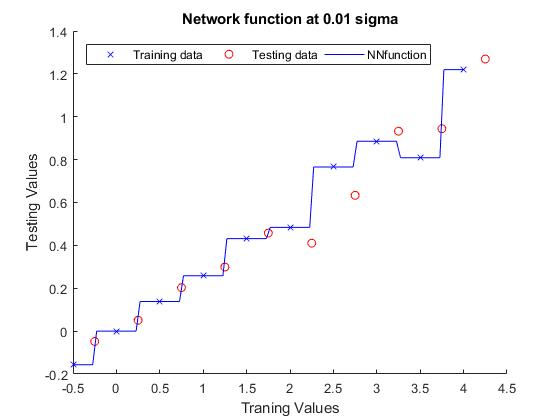
\includegraphics[scale = 0.35]{NNstepfunction.jpg}
\vspace{1.5mm}
{\footnotesize figure 7 : Network function when sigma is 0.01 }
\\
\vspace{1.5mm}
\end{flushleft}
\begin{flushleft}
  Once the network was working properly, the sigma optimiation could begin to see which sigma would be best to use for the
  network. To do this the network was run over the data set 100 times and then the final test and train error where taken and
  stored. This allowed for the best value on the testing data to be found. The sigma was tested between 0.1 - 1 and the table
  of results can be seen in figure 10. The best sigma value that could be found from this testing was 0.9 as it had the lowest
  test error of all of the value tried with a error value of 0.0915. The error graph and network function graph for this sigma
  can be seen in figure 8 and 9.
  \\
\vspace{1.5mm}
\begin{center}
  Error plot for a sigma of 0.9
\end{center}
\vspace{1.5mm}
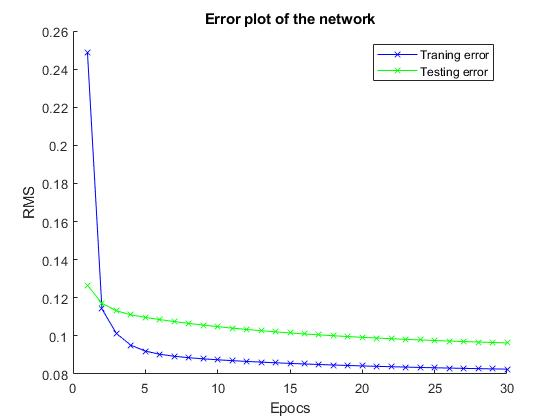
\includegraphics[scale = 0.35]{Errorplottask1.jpg}
\vspace{1.5mm}
{\footnotesize figure 8 : error plot for the network with sigma 0.9 }
\\
\vspace{1.5mm}
\begin{center}
  Network function plot for a sigma of 0.9
\end{center}
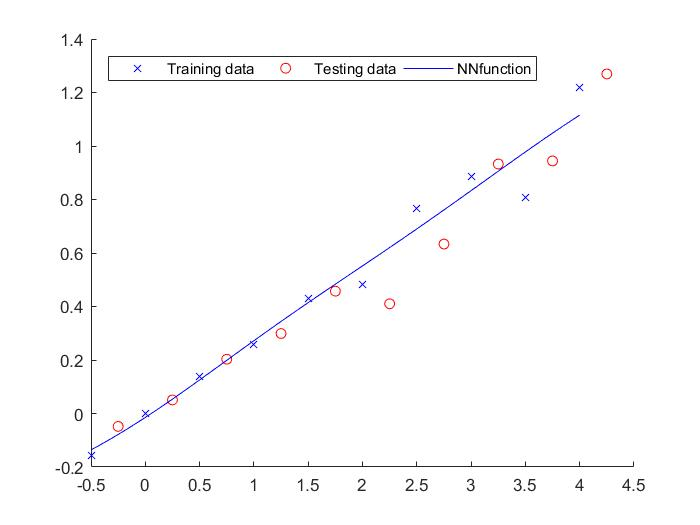
\includegraphics[scale = 0.35]{NNfunctiontask1.jpg}
\vspace{1.5mm}
{\footnotesize figure 9 : Network function when sigma is 0.9 }
\\
\vspace{1.5mm}
\end{flushleft}
\begin{center}
\begin{tabular}{||c c c||}
  \hline
Sigma Value & Train Error & Test Error \\ [0.5ex]
\hline
0.1 & 0.2733e-16 & 0.1005\\
0.2 & 2.0126e-10 & 0.1016\\
0.3 & 1.3562e-4 & 0.1094\\
0.4 & 0.0131 & 0.1161 \\
0.5 & 0.0439 & 0.1073 \\
0.6 & 0.0632 & 0.0983\\
0.7 & 0.0730 & 0.0933\\
0.8 & 0.0781 & 0.0919\\
0.9 & 0.0797 & 0.0915\\
1.0 & 0.0800 & 0.0918\\
\hline
\end{tabular}
\end{center}
\vspace{1.5mm}
{\footnotesize figure 10 : Sigma optimisation table }
\\
\vspace{1.5mm}
\subsubsection{Tast 2}
\begin{center}
\begin{tabular}{||c c c||}
  \hline
Number of Nodes & Train Error & Test Error \\ [0.5ex]
\end{tabular}
\end{center}
\begin{center}
\begin{tabular}{||c c c||}
  \hline
Sigma Value & Train Error & Test Error \\ [0.5ex]
\hline
0.1 \\
0.2 \\
0.3 \\
0.4 \\
0.5 \\
0.6 \\
0.7 \\
0.8 \\
0.9 \\
1.0 \\
\hline
\end{tabular}
\end{center}
\subsection{MLP}
\subsubsection{Task 2}
\section{Data}
\subsection{Data processing methods}
\subsection{Problems with the data}
\section{results}
\section{conclution}
\end{document}
